\documentclass[12pt letterpaper]{article}

\usepackage{fullpage}
\usepackage{graphicx}
\usepackage{amsmath}

\providecommand{\e}[1]{\ensuremath{\times 10^{#1}}}
\usepackage{gensymb}

\usepackage{float}


\title{Chaos In the Diode-R-L Circuit}
\author{Johnny Minor \\ Partner: Kayla Mitchell}
\date{\today}

\begin{document}

\maketitle

%abstract should have a very brief overiew of the goals and main results of the experiment. 
\begin{abstract}
In this experiment we used a diode, resistor, inductor circuit to study the non linear behavior of the diode. We powered the circuit at it's natural frequency with a sinusoidal voltage. We then incremented the voltage amplitude and observed the behavior of the voltage across the diode on an oscilloscope. Since the diode is non linear we were able to find experimentally the bifurcations of the diode. These three bifurcations were printed off for later viewing. Furthermore, the voltage was increased past the third bifurcation and the system clearly became chaotic as we could see jumps and non linear spikes of voltage on the oscilloscope. The Feigenbaum number was then calculated. Our experimental values confirmed the expected Feigenbaum number of 4.66. 
\end{abstract}

\newpage

\section*{Description of Experiment}

When we replace a the capacitor in the familiar RLC (Resistor Inductor Capacitor) with a diode it can exhibit bifurcation and with a high enough amplitude chaos too. This is because the diode is non linear. Non linear behavior comes about all over in the natural world. From weather patterns, to ocean currents, and population growth. These can non linear behaviors can be modeled using a map.  So, the purpose of this experiment was to study period doubling in a circuit and also the determination of the Feigenbaum number. 

\begin{figure}[H]
  \caption{The experimental setup as a circuit diagram.}
  \centering
    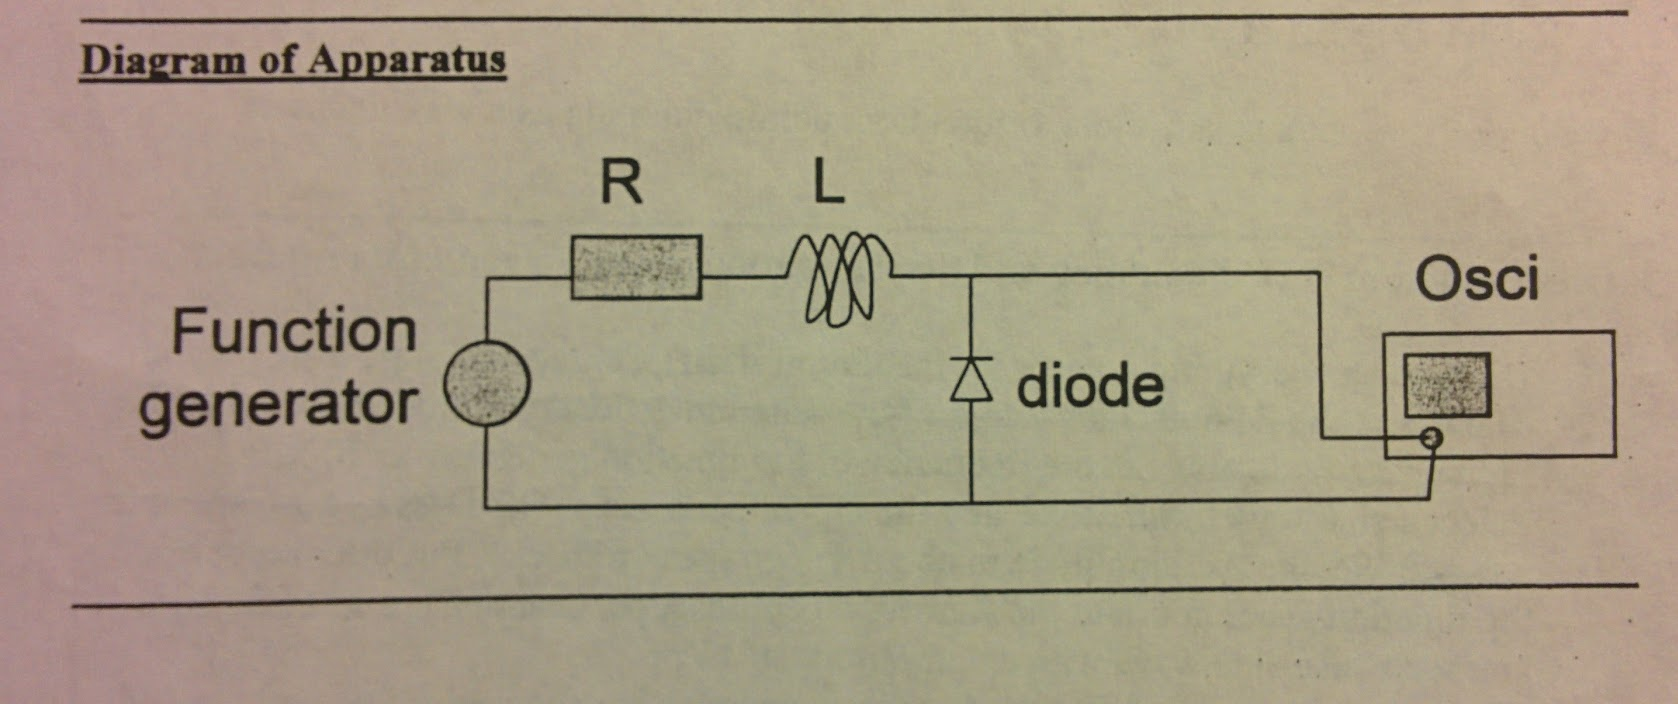
\includegraphics[width=.60\textwidth]{circuit_chaos.jpg}
    \label{fig:circuit}
\end{figure}

Mitchell Feigenbaum is a mathematical physicist who studied chaotic systems. What he discovered in 1975 was that all systems that exhibit chaos with the difference $\Delta_n = \lambda_{n+1} - \lambda_n$ of the values when bifurcation occurs rapidly converges as $n$ approaches infinity. If we take a ratio of these differences between each bifurcation interval and the next we come to Feigenbaum constants. 

\begin{equation}
\label{feigenbaum}
\delta = \lim_{n\rightarrow \infty} \frac{a_{n-1} - a_{n-2}}{a_n - a_{n-1}} = 4.669\,201\,609\,\cdots
\end{equation}

where $a_n$ are values, in our case the voltage, at the $n$th period doubling. So, we would expect to find be able to confirm this value in our own experiment. 

In the experiment we first used the Kenwood oscilloscope to check that our output voltage was set correctly. We set the frequency generator to a sine waveform at 70 kHz with no DC offset and the AC amplitude was set to 1 Vpp (Volt peak to peak). We then varied the voltage on the function generator by 0.01 V which was the minimum possible with the function generator. Once the period doubling was observed we noted at which amplitude and then looked at when the period doubling was able to seen to get a handle on the error. 


\section*{Data and Analysis}

The raw data which we collected can be seen clearly in table \ref{table:data}. In each case our error was $\pm0.05$V. 
It was difficult to get a clear view of exactly when the bifurcation occurred. Especially between the third period doubling and the chaotic region. So this seems reasonable error. 

\begin{table}[H]
\centering
\caption{The data for the bifurcations we observed.}
\label{table:data}
\begin{tabular}{|l|l|}
\hline
Bifurcation & AC Amplitude (Vpp) \\ \hline
1st         & 2.6                \\ \hline
2nd         & 3.50                \\ \hline
3rd         & 3.70                \\ \hline
Chaos       & 3.80                \\ \hline
\end{tabular}
\end{table}


\begin{figure}[H]
  \caption{Oscilloscope print off with 1.0 Vpp. }
  \centering
    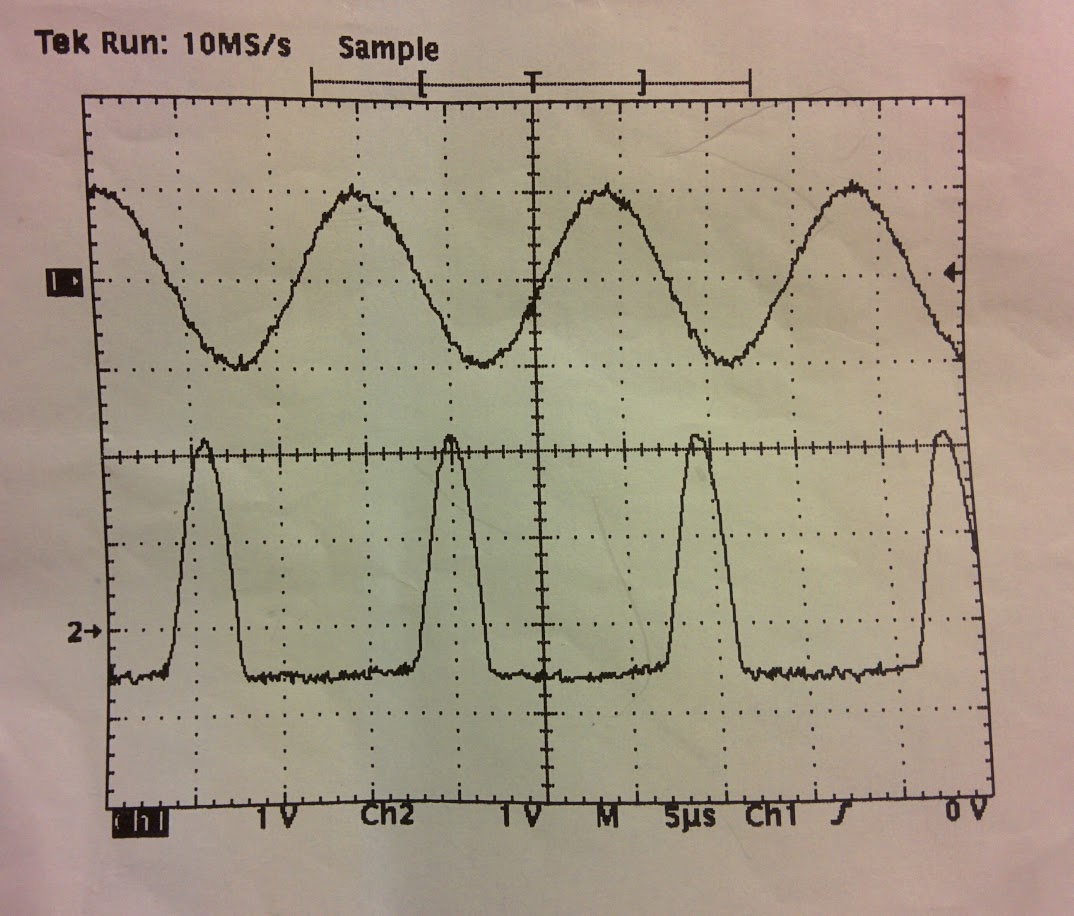
\includegraphics[width=.60\textwidth]{normal_diode.jpg}
    \label{fig:normal}
\end{figure}

Our plot looks like this because we are driving the circuit at it's natural frequency, and also because we don not have a period doubling taking place. This happens because the driving voltage goes negative which in turn flips the diode. So then the diode will block the voltage and we see zero voltage. 


\begin{figure}[H]
  \caption{Oscilloscope print off showing the first period doubling.}
  \centering
    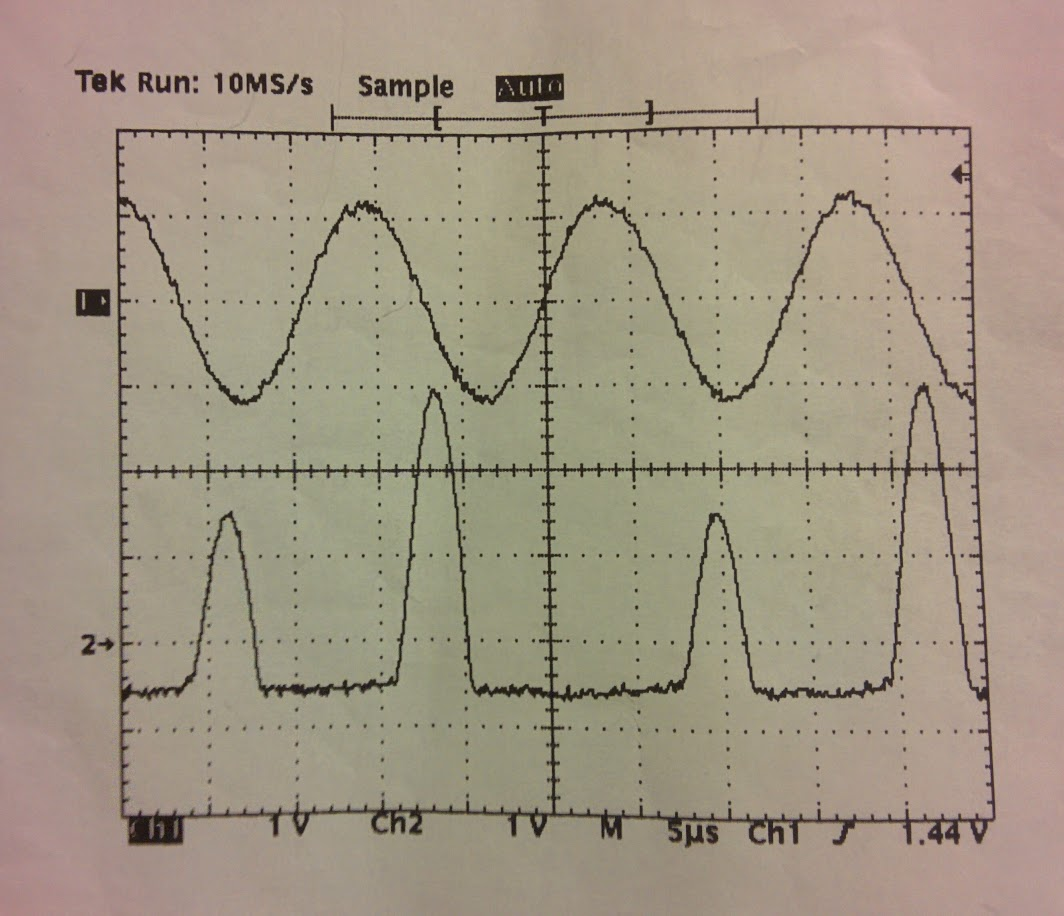
\includegraphics[width=.60\textwidth]{first_doubling.jpg}
    \label{fig:first}
\end{figure}

This is what we identified as the second period double. We saw this on the oscilloscope at 2.6$\pm0.05$ Vpp. 

\begin{figure}[H]
  \caption{Oscilloscope print off showing the second period doubling.}
  \centering
    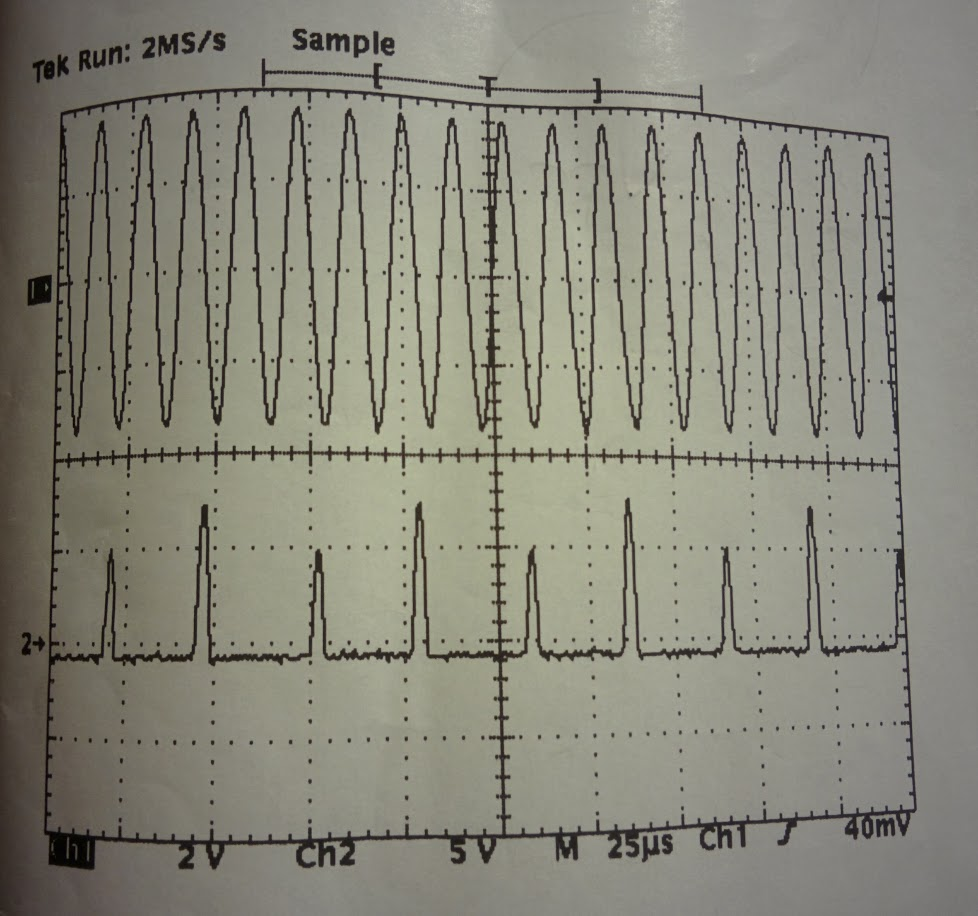
\includegraphics[width=.60\textwidth]{second_doubling.jpg}
    \label{fig:second}
\end{figure}

This is what we identified as the second period double. We saw this on the oscilloscope at 3.5$\pm0.05$ Vpp. 

\begin{figure}[H]
  \caption{Oscilloscope print off showing the third period doubling.}
  \centering
    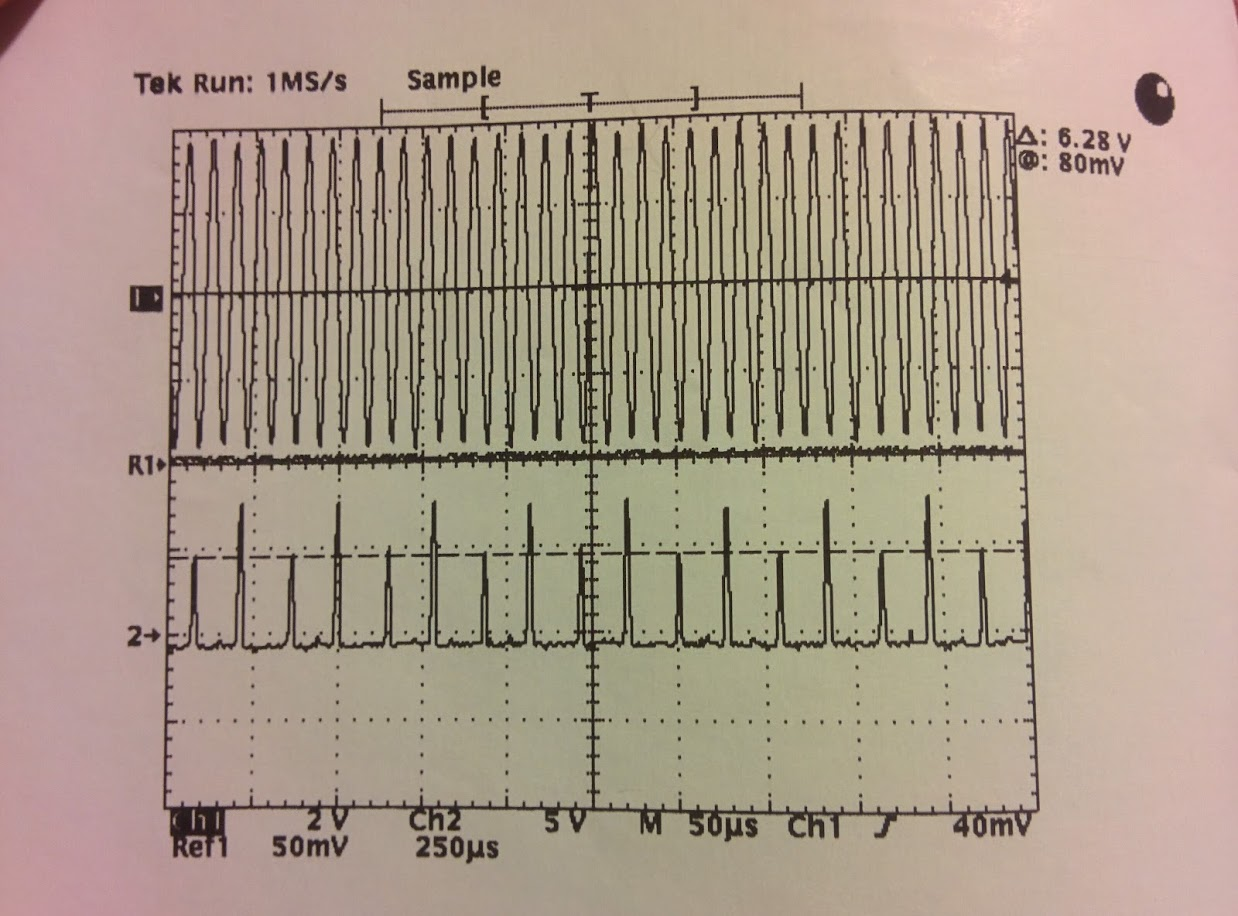
\includegraphics[width=.60\textwidth]{third_doubling.jpg}
    \label{fig:third}
\end{figure}

Although it can't be seen easily in figure \ref{fig:third} as we slightly increased the voltage on the frequency generator the peaks began to wiggle. This is because we were beginning to see the chaotic nature of the diode. Looking on the Kenwood oscilloscope this is very apparent because the Kenwood oscilloscope draws over the past periods. Therefore, some of the lines end up looking wiggly and thicker because of the overlap of lines being drawn on top of each other. When we switched to the Tektronix oscilloscope this wiggling wasn't apparent because 

\begin{figure}[H]
  \caption{Oscilloscope print off showing the beginning of the chaotic region.}
  \centering
    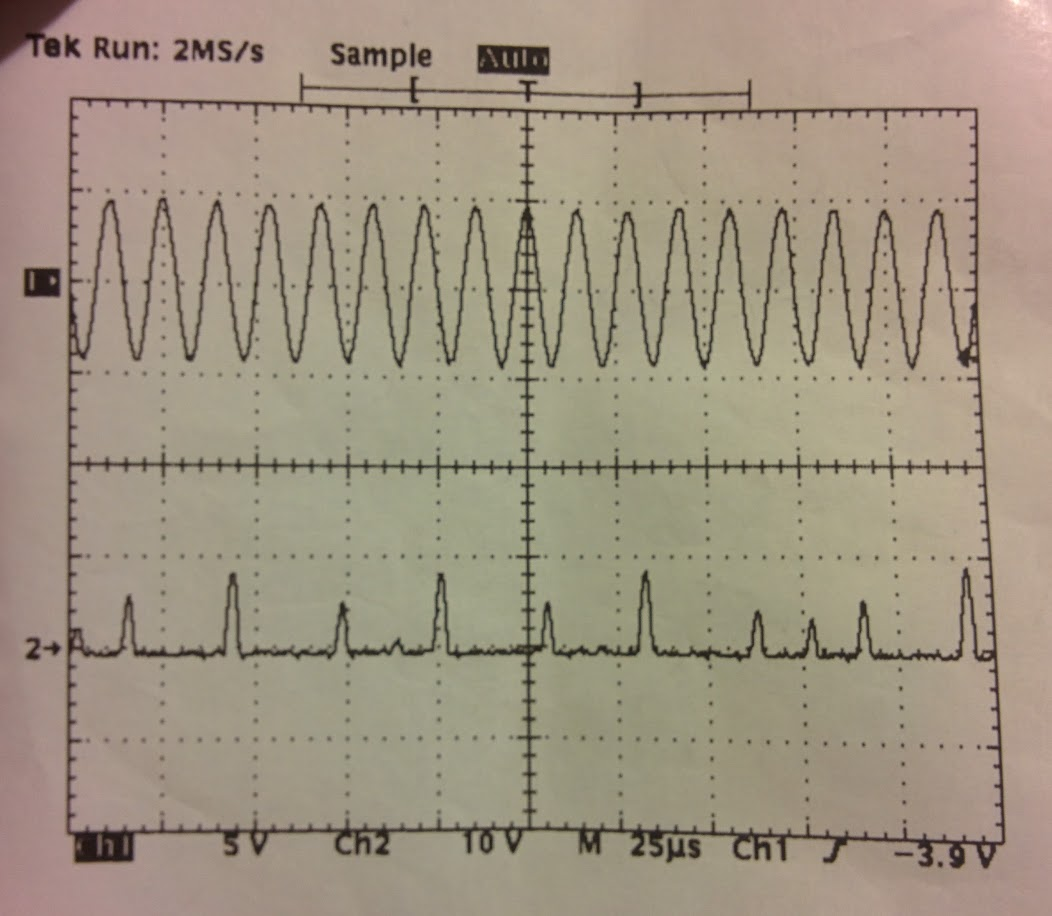
\includegraphics[width=.60\textwidth]{chaos.jpg}
    \label{fig:chaos}
\end{figure}

This is what we saw on the oscilloscope at 3.8$\pm0.05$ Vpp. 



\section*{Results and Conclusions}

Finally, we would like to calculate the Feigenbaum number with our data in table \ref{table:data}. 
$$ 
\lambda_2 - \lambda_1 =  0.90\pm0.05 \mathrm{V} 
$$
$$ 
\lambda_3 - \lambda_2 = 0.20\pm0.05 \mathrm{V}
$$

So then the Feigenbaum number we calculate is 

$$ 
\delta = \frac{\lambda_2 - \lambda_1}{\lambda_3 - \lambda_2} = 4.60 \pm 0.10 
$$

This seems to agree with our expected value we found in equation \ref{feigenbaum}. 

In this experiment we found and confirmed the three period doubling points in our RLD circuit. Our calculated Feigenbaum number agrees with what we would expect which gives us confidence in our experimental data. 


\end{document}